\documentclass[a4paper]{article}

%% Language and font encodings
\usepackage[brazil,english]{babel}
\usepackage[utf8]{inputenc}
%% Sets page size and margins
\usepackage[a4paper,top=3cm,bottom=2cm,left=3cm,right=3cm,marginparwidth=1.75cm]{geometry}

%% Useful packages
\usepackage{amsmath}
\usepackage{graphicx}
\usepackage[colorinlistoftodos]{todonotes}
\usepackage[colorlinks=true, allcolors=blue]{hyperref}
\usepackage{listings}
\usepackage{color}
\lstset{ %
  language=R,                     % the language of the code
  basicstyle=\footnotesize,       % the size of the fonts that are used for the code
  numbers=left,                   % where to put the line-numbers
  numberstyle=\tiny\color{gray},  % the style that is used for the line-numbers
  stepnumber=1,                   % the step between two line-numbers. If it's 1, each line
                                  % will be numbered
  numbersep=5pt,                  % how far the line-numbers are from the code
  backgroundcolor=\color{white},  % choose the background color. You must add \usepackage{color}
  showspaces=false,               % show spaces adding particular underscores
  showstringspaces=false,         % underline spaces within strings
  showtabs=false,                 % show tabs within strings adding particular underscores
  frame=single,                   % adds a frame around the code
  rulecolor=\color{black},        % if not set, the frame-color may be changed on line-breaks within not-black text (e.g. commens (green here))
  tabsize=2,                      % sets default tabsize to 2 spaces
  captionpos=b,                   % sets the caption-position to bottom
  breaklines=true,                % sets automatic line breaking
  breakatwhitespace=false,        % sets if automatic breaks should only happen at whitespace
  title=\lstname,                 % show the filename of files included with \lstinputlisting;
                                  % also try caption instead of title
  keywordstyle=\color{blue},      % keyword style
  commentstyle=\color{teal},   % comment style
  stringstyle=\color[rgb]{1,0,0},      % string literal style
  escapeinside={\%*}{*)},         % if you want to add a comment within your code
  morekeywords={*,...}            % if you want to add more keywords to the set
}

\addto\captionsenglish{\renewcommand{\figurename}{Figura}}
\renewcommand{\lstlistingname}{Código}

\title{Estatísticas para um Melhor Desempenho no League of Legends}
\author{Iverson Pereira e Ricardo Luna}

\begin{document}
\maketitle

\begin{abstract}
Your abstract.
\end{abstract}

\section{Introdução}

\textit{League of Legends} ou popularmente conhecimento como LoL é um jogo disponível online estilo MOBA (\textit{Multiplayer Online Bale Arena}) e também possui fortes elementos de RPG (\textit{Role-Playing Game}). Dentre outras características o jogo tem apresentado dados bastantes significativos nos últimos anos. Em 2017, o cenário competitivo teve um faturamento de U\$12,016,606.24 como um total de 135 campeonatos nesse período o que representa um dos maiores faturamentos em jogos desse estilo.  

O jogo teve sua inspiração em outro jogo chamado Dota (\textit{Defense of the Ancients}). Dota tem como objetivo a destruição de uma estrutura principal para condição de vitória da partida. Essa estrutura de jogo também é comum ao LoL com adição de outros elementos próprios: rota de selva, dragões elementais e outros recursos que fornecem maiores vantagens para equipe.  

O jogo tem apresentado aspectos bastantes interessantes mais recentemente, a cada nova sessão, atualização grande que traz mudanças maiores ao jogo, ou a cada novo \textit{patch} que são atualizações menores visando o balanceamento e resolver problemas no jogo. Isso possibilita que jogadores mais experientes descubram ou proponham novas formas de jogo e composições objetivando um melhor desempenho e consequentemente aumentando suas chances de vitória. 


Assim como mostrado na Figura~\ref{fig:map}, o jogo possui quatro rotas: \textit{top} (superior), \textit{mid} (meio), bot (inferior) e \textit{jungle} (selva). Cada uma dessas rotas possui uma característica própria e com isso o os personagens que jogam nessas rotas devem cumprir certos requisitos.  No topo é utilizando normalmente um personagem capaz que ficar vivo durante um longo tempo nas lutas e sofre boa parte do dano que seria direcionado aos jogadores de seu time. Já na rota do meio, geralmente são utilizados personagens com um dano por segundo (\textit{dps}) alto e assim eliminar os jogadores do time inimigo que possam causar mais dano ao seu time. Os jogadores da rota inferior, que são geralmente dois, são o ADC (\textit{Attack Damage Carry}), que tem como função causar grandes cargas de dano ao time inimigo e geralmente esses personagens possuem ataque a longa distância, e o suporte é o responsável por manter o ADC vivo, geralmente deve possuir habilidades para auxiliar os outros jogadores como curas, escudos e controles de grupo visando causar algum atraso ou retardar o ataque da equipe inimiga. 

\begin{figure}[ht]
\centering
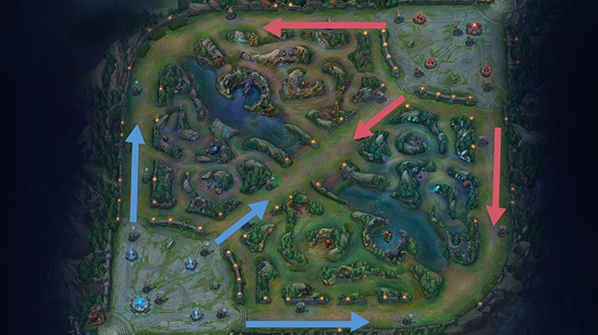
\includegraphics[width=0.7\textwidth]{imagens/rotas}
\caption{\label{fig:map}Mapa do Summoner's Rift.}
\end{figure}

Mas como já mencionado o jogo vem trazendo mudanças mais frequentes e isso tem ``forçado" uma adaptação mais rápida de seus jogadores. O META, como essa adaptação é chamada, pode ser visto como um estilo que ao longo do tempo vem se mostrando mais efetivo que os outros e aproveita mais efetivamente os recursos disponíveis. Mas a pergunta que fica é ``como se adaptar de forma mais rápida ao META?".  Diante deste questionamento, este trabalho tenta trazer uma resposta. De forma simples o trabalho mostra uma análise baseada em estatísticas do jogo visando mostrar quais os personagens estão mais fortes, no \textit{patch} atual, ou quais personagens melhor se adaptam ao novo META.  

O projeto deve utilizar uma base de dados retirada do site OP.GG\footnote{http://br.op.gg/}. Esta base de dados possui um histórico de todas as partidas realizadas no jogo e outras informações relacionadas. Com um total de mais de 12 mil partidas, os dados representam informações cruciais do jogo. Listamos abaixo estas informações: 

\begin{itemize}
	\item Personagens utilizados em cada equipe;
    
	\item Resultado final da partida, derrota ou vitória;
    
    \item Liga, que indica qual o ``nível" ou ranking dos jogadores;
    
    \item \textit{Patch} no qual o jogo foi realizado;
    
    \item Região onde ocorreu o jogo.
\end{itemize}  


O trabalho deve oferecer um conjunto de estatísticas que serão descobertas a partir dos dados. Dentre elas, propomos estatística para taxa de vitória por personagem, popularidade de cada personagem por região (baseado na quantidade de partidas jogadas) e também o uso do k-NN (\textit{k-Nearest Neighbors}). O uso do k-NN tem a finalidade de prever o time vencedor utilizando dois times como entrada para o algoritmo. Esta previsão é baseada na análise do conjunto de dados estatísticos gerado, para que se possa afirmar quais composições terão maiores chances de ganhar ou não uma partida. Diante disso, o jogador pode utilizar essas informações baseadas em estatística para auxiliá-lo e, dessa forma, obter um maior conhecimento sobre o jogo de forma rápida e confiável.

\section{Pacotes Requeridos}

Para executar essa análise é preciso instalar e carregar alguns pacotes específicos que não são nativos em R. Os pacotes utilizados para essa análise de dados estão dispostos no Código~\ref{cod:library}. O pacote \texttt{tidyr} é utilizado para ajustar tabelas, como por exemplo, transformar colunas em linhas com o comando \texttt{gather}. O pacote \texttt{dplyr} é usado para manipulação dos dados para facilitar a obtenção de informações com o uso de funções como \texttt{group\_by} e \texttt{summarise}. A biblioteca \texttt{stringr} é importada para auxiliar em operações com \textit{strings}.

\begin{lstlisting}[language=R, caption={Pacotes utilizados no projeto},label={cod:library}]
#Carrega os pacotes necessarios
library(tidyr) #Ajustar os dados
library(dplyr) #Manipular os dados
library(stringr) #Operacoes com string
\end{lstlisting}

\section{Preparação dos Dados}

\subsection{Fontes dos dados}
Para a obtenção da base de dados utilizamos um projeto do GitHub chamado LOL.tools\footnote{em https://github.com/MarcusDEFGH/LOL.tools}. Este projeto utiliza o Scrapy\footnote{https://scrapy.org/}, biblioteca em Python, que coleta os dados de uma página web e gera um arquivo .\texttt{csv} com os dados capturados. O site de onde os dados são extraídos é o OP.GG. Como já mencionado esse site disponibiliza um histórico de todas as partidas do jogo e tal dado é divido por regiões, onde cada região representa os servidores implantados.

\subsection{Entendendo os Dados}
Os dados coletados são relacionados as ligas do disponíveis no jogo (bronze, prata, ouro, platina, diamante, mestre e desafiante), cada liga representa um nível de habilidade do jogador. Para ser classificado a um liga, o jogador deve jogar 10 partidas e a partir do seu desempenho o jogador será classificado. Todos as ligas começam no nível 5 e vão no máximo até o 1. Para subir entre os níveis, de uma mesma liga, o jogador deve jogar 3 partidas, quando atingir o limite de 100 Pontos de Liga (PdL), se obtiver duas vitórias o jogador é promovido. Para conseguir subir de liga o jogador deve chegar no nível 1 da liga e obter 100 PdL e caso consiga vencer 3 das 5 partidas que devem ser disputadas o jogador é promovido. Quando se chega no ouro o jogador ganha um conjunto de itens dentro do jogo a cada sessão, geralmente no início do ano, e ao se chegar no desafiante o jogo envia presentes para os jogadores de cada região. Geralmente nas equipes competitivas os jogadores escolhidos são do nível desafiante e a premiação é maior nos campeonatos. 

Os dados assim que coletados apresentam um total de 14 colunas, ilustrado na Figura~\ref{fig:dataantes}. As 10 primeiras colunas representam os integrantes (personagens) dos times. Os personagens do primeiro time são representados pelos valores das colunas $team_1.x$, onde x varia de 0 até 4.  Os personagens do time 2 são representados pelas colunas $team_2.x$, análogo ao time 1. Para cada um desses times temos um total de 143 possíveis personagens disponíveis para a escolha do jogador, mas como o modo de jogo é dividido por ranking desse total 10 personagens são banidos antes do início da partida. Esse banimento é usado para remover personagens que se mostraram fortes no \textit{patch} atual ou caso um jogador possa ter um nível muito alto de habilidade com o mesmo.

\begin{figure}[ht]
\centering
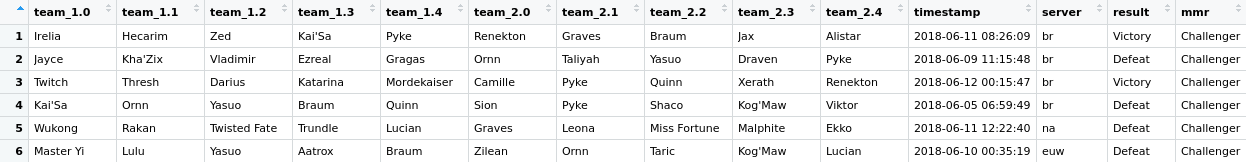
\includegraphics[width=15cm]{imagens/data_before}
\caption{\label{fig:dataantes}Conjunto de dados coletados}
\end{figure}

A coluna \textit{timestamp} representa a data e horário do término da partida e não fui utilizado na análise dos dados. A coluna \textit{server} indica a região onde a partida foi realizada (BR, EUNE, EUW, JP, LAN, LAS, NA, OCE, RU, TR). A coluna \textit{result} indica o resultado do jogo mas apenas com relação ao primeiro time, no caso o valor deve ser invertido para o time 2. Por fim, a coluna mmr indica o ranking da partida armazenada (\textit{MatchMaking Rate} - MMR). 

\subsection{Formatação e Limpeza}

Após o carregamento dos dados, percebemos que seria importante a junção dos personagens de cada time em uma única coluna. Isto é, para o time 1, haveria uma coluna com os cinco personagens escolhidos, por sua vez, o time 2 também teria essa mesma representação em uma outra coluna. Diante disso, inicialmente concatenamos as variáveis que apresentam o nome dos personagens de cada time. Para tal etapa foi utilizada a função \texttt{unite} com o separador “\_”, como ilustrado no Código~\ref{cod:readdata}. Essa etapa foi realizada visando a simplificação das operações que podem ser realizadas usando as operações entre \textit{strings} contidas no R. O segundo tratamento efetuado é a mudança do valor na variável \texttt{result}, que poderia ser \texttt{Victory} ou \texttt{Defeat}, para um valor booleano como \textit{True} ou \textit{False}. Essa operação simplifica qualquer outra operação futura pois esse valor poder ser facilmente convertido para inteiro e assim efetuar operações de soma ou média que serão utilizadas no projeto. Durante a leitura dos dados foi utilizada a função \texttt{read.csv} com todos os parâmetros padrões do R e o adiciona de \textit{stringsAsFactors} como falso. A Figura \ref{fig:data_clean} mostra o resultado obtidos após a limpeza dos dados, as colunas exibidas são: $team_1$, $team_2$, $server$, $result$ e $mmr$.

\begin{lstlisting}[language=R, caption={Leitura da base de dados},label={cod:readdata}]
dados<-read.csv('patch811.csv', stringsAsFactors = F)

# Concatena os valores das variaveis team1.x
dados<-dados %>%
  unite(col = "team_1",
        1,2,3,4,5,
        sep = "_")
        
# Concatena os valores das variaveis team2.x
dados<-dados %>%
  unite(col = "team_2",
        2,3,4,5,6,
        sep = "_")
\end{lstlisting}


\begin{figure}[ht]
\centering
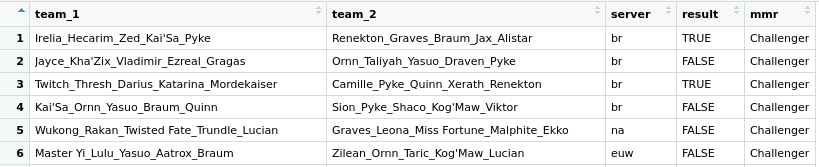
\includegraphics[width=15cm]{imagens/clean_data2}
\caption{\label{fig:data_clean}Dados após a limpeza}
\end{figure}

A Figura \ref{fig:names} mostra o nomes de todos os personagens do jogo até o \textit{patch} $8.14$ e sendo assim todos os nomes possíveis para a composição de ambos os times. 


\begin{figure}
\centering
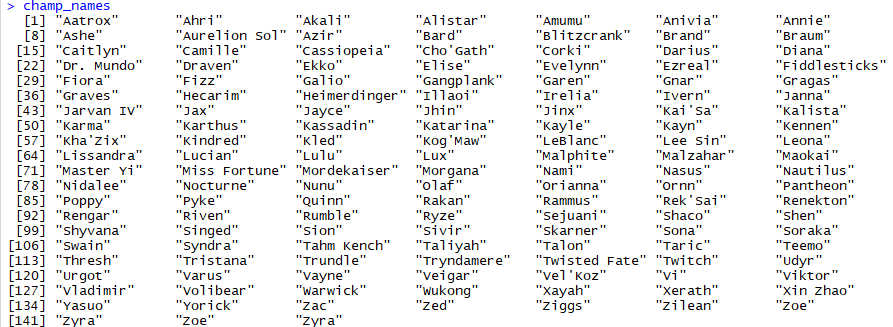
\includegraphics[width=15cm]{imagens/champ_names}
\caption{\label{fig:names}Nome dos personagens do jogo}
\end{figure}

\section{Análise Exploratória}


Dado o conjunto de dados é possível extrair informações que antes não estava tão evidentes, informação como a taxa de vitória de uma personagem, podendo ser obtida de forma global (todas as regiões) ou local, e a popularidade de um personagem.

A taxa de vitória de um personagem pode ser algo associado ao \textit{patch} atual ou a popularidade dele, normalmente quando são feitos pequenos ajustes no jogo ou balanceamentos alguns dos personagens podem ganhar um pico de poder se comparado a sua versão antiga. Ou fator que pode influenciar nessa medida é o nível de dificuldade atrelado ao aprendizado com o uso de um certo personagem, certos personagens oferecem mecânicas mais simples e outros mais complexas. Quando um jogador mais experiente, geralmente nos ligas mais altas do jogo, ele possui certa facilidade com as mecânicas do jogo e esse fator quando aplicado em um personagem que está em seu pico de poder a taxa de vitória aumenta consideravelmente. 

No jogo a equipe SKT T1 da Coreia do Sul já foi considerada a melhor do mundo, nessa região o nível dos jogadores do competitivo é realmente alto se comparado com outras regiões. O jogador Faker (Lee Sang-hyeok), que joga no meio, já foi considerado por muitos anos o melhor jogador em sua posição. Esse jogador tem um alto nível e quando em uma de suas partidas, seja em competições ou em partidas solo, e quando mostra um bom desempenho com algum personagem do jogo outros jogadores do mundo tentam “copiar” seu estilo de jogo, que se mostrou extremamente eficaz, e assim surgem os METAS.


Já que os dados apresentam um conjunto de combinações de times e o resultado da partida é possível aplicar algoritmos como KNN (\textit{K nearest neighboors}) \cite{fukunaga1975branch}. Sua ideia principal é que possível estimar uma classe de um novo dado baseado no conjunto de vizinhos obtidos a partir de uma análise na base de dados. Para se estimar qual o nível de similaridade com um determinando elemento é utilizada uma função. Como os dados da base são apenas nomes dos personagens o calculo é realizado utilizando quantos \textit{matchs} foram obtidos entre um time e toda a base dados. O resultado da partida, que pode ser vitória ou derrota, será obtido como a classe que foi associada a maioria dos vizinhos desse objeto avaliado. 


A Figura \ref{fig:win_rate} mostrar as melhores taxa de vitórias e pior taxa de vitórias, usando o comando head() e tail() respectivamente, as barras indicam a taxa de vitória e a legenda mostra qual os seus valores utilizando as cores como referência. Com os dados apresentando nessa figura é possível observar que os personagens Quin, Pantheon, Poppy, Cassiopeia e Kog’Maw obtêm os melhores rates, de forma global. Enquanto, Jinx, Amumu, Volibear, Tristana, Xerath e Elise apresentam os piores resultados. 

\begin{figure}
\centering
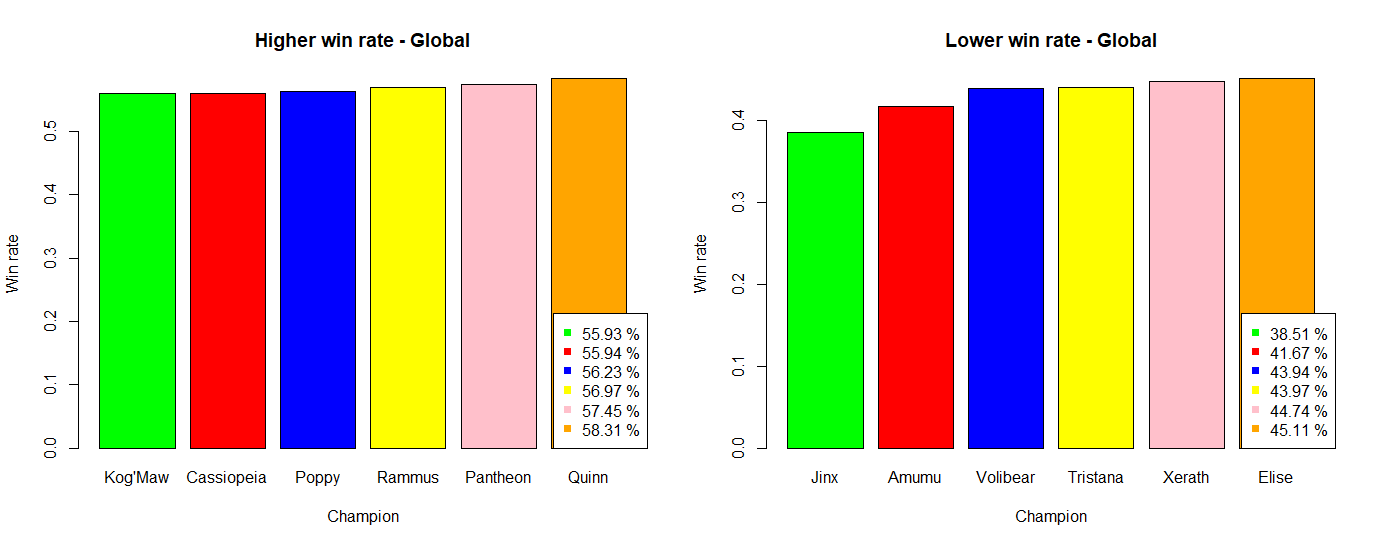
\includegraphics[width=0.7\columnwidth]{imagens/Rplot}
\caption{\label{fig:win_rate}Taxa de vitórias global.}
\end{figure}

Os dados mostram que se um jogador for iniciar uma partida ou tentar melhorar com um novo personagem seria interessante observar jogos de um jogador mais experiente, facilmente encontrados no \textit{Youtube} ou \textit{Twitch tv}, e depois que entender a mecânica desse personagem inicia seus treinos. Usando uma estratégia assim o jogador pode atingir maiores taxa de vitória e usar o \textit{META} e as estatística a seu favor.

\section{Conclusões}



\bibliographystyle{alpha}
\bibliography{sample}

\end{document}